\documentclass[11pt]{article}
\usepackage{tocloft}
\usepackage{graphicx}
\usepackage{calc}
\usepackage{amssymb}
\usepackage{amsmath}
\usepackage{color}
\usepackage[sc]{mathpazo}
\usepackage{url}

\def\LL{\left\langle}   % left angle bracket
\def\RR{\right\rangle}  % right angle bracket
\def\LP{\left(}         % left parenthesis
\def\RP{\right)}        % right parenthesis
\def\LB{\left\{}        % left curly bracket
\def\RB{\right\}}       % right curly bracket
\def\PAR#1#2{ {{\partial #1}\over{\partial #2}} }
\def\PARTWO#1#2{ {{\partial^2 #1}\over{\partial #2}^2} }
\def\PARTWOMIX#1#2#3{ {{\partial^2 #1}\over{\partial #2 \partial #3}} }

\def\rightpartial{{\overrightarrow\partial}}
\def\leftpartial{{\overleftarrow\partial}}
\def\diffpartial{\buildrel\leftrightarrow\over\partial}

\def\BC{\begin{center}}
\def\EC{\end{center}}
\def\BN{\begin{enumerate}}
\def\EN{\end{enumerate}}
\def\BI{\begin{itemize}}
\def\EI{\end{itemize}}
\def\BE{\begin{displaymath}}
\def\EE{\end{displaymath}}
\def\BEA{\begin{eqnarray*}}
\def\EEA{\end{eqnarray*}}
\def\BNEA{\begin{eqnarray}}
\def\ENEA{\end{eqnarray}}
\def\EL{\nonumber\\}


%\linespread{1.05}
\oddsidemargin=0pt
\evensidemargin=0pt
\textwidth=6.5in
\topmargin=0pt
\headheight=0pt
\headsep=0pt
\textheight=9in
% EXPERIMENTAL
%\parindent=0pt
%\parskip=3pt
\setlength{\parindent}{0cm}
\newcommand\secfont{\fontfamily{cmss}\selectfont}%\textwidth 5.5truein
\newcommand\pifheading[1]{{\secfont\textbf{#1}:}}
%\oddsidemargin -0.40truein
%\textheight 8.0truein
%\topmargin -0.25truein
\def\lo{
\mathrel{\raise.3ex\hbox{$<$}\mkern-14mu\lower0.6ex\hbox{$\sim$}}
}
\def\hi{
\mathrel{\raise.3ex\hbox{$>$}\mkern-14mu\lower0.6ex\hbox{$\sim$}}
}

\textwidth = 6.6 in
\textheight = 9.1 in
\oddsidemargin = -0.05 in
\evensidemargin = +0.05 in
\topmargin = -.1 in
\headheight = 0.0 in
\headsep = 0.0 in
\parskip = 0.06in
\newcommand\registered{{\ooalign{\hfil\raise .00ex\hbox{\scriptsize R}\hfil\crcr\mathhexbox20D}}}

%% Define a new 'leo' style for the package that will use a smaller font.
\makeatletter
\def\url@leostyle{%
  \@ifundefined{selectfont}{\def\UrlFont{\sf}}{\def\UrlFont{\small\ttfamily}}}
\makeatother
%% Now actually use the newly defined style.
\urlstyle{leostyle}

%\pagestyle{empty}
%\includeonly{previous,proposal_references}
%\includeonly{proposal_references}
%\includeonly{previous}

% TOC

\begin{document}
%%%%%%%%%%%%%%%%%%%%%%%%%%%%%%%%%%%%%%%%%%%%%%%%%%%%%%%%%%%%%%%%%%%%%
\begin{center}
\textbf{\Huge
Lab 9: How hot are the planets?\\
\vspace*{0.1cm}
}
\end{center}

\vspace*{0.5cm}

{\Large Name:}\vspace*{0.5cm}\\\hrule
{\Large NetID:}\vspace*{0.5cm}\\\hrule
{\Large Lab section number:}\vspace*{0.5cm}\\\hrule


%%%%%%%%%%%%%%%%%%%%%%%%%%%%%%%%%%%%%%%%%%%%%%%%%%%%%%%%%%%%%%%%%%%%%
\section{Introduction}

\subsection*{Foreword}

In this lab, you and your group
will use the physics of thermal radiation to estimate the temperatures of various planets in the Solar System. We will return
to the results of this lab multiple times in class, so it's important that you understand the takeaway message from this lab
when you leave today.

You will be working with mathematics -- algebra and numbers. While we know that your mathematics backgrounds vary greatly, the only skills you will need for this lab are
high school algebra, a little arithmetic, and a bit of geometry. This lab involves no computer simulations, lab equipment, or materials -- it is a calculation that you will do using
pencil and paper (and, likely, a calculator).

Do not be intimidated by the fact that ``I am making you do math''; this lab handout walks you through the calculation, and you have your lab group and your TA to help you.

\subsection*{Background: the Stefan-Boltzmann law and temperature}

As you learned in class, objects with a temperature emit light called {\it thermal radiation}. We discussed that, as an object's temperature increases...

\BI
\item The peak wavelength of the light emitted gets shorter
\item The total amount of light emitted increases rapidly
\EI

In this lab, we care only about this second property. For this lab, we will need a mathematical expression of this idea, called the {\it Stefan-Boltzmann law}.

This law says:

\begin{center}

{\bf If an object has a temperature $T$, that object's surface\\ shines with an intensity of $I=kT^4$.}

\end{center}

Here $k$ is a mathematical constant; you do not need its value and can leave it in your algebraic expressions, as it will wind up cancelling out in the end. 

It is important here that the temperature $T$ be measured in the Kelvin scale. You may convert temperatures in Kelvin to Fahrenheit or Celsius as follows:

\BI
\item T (Celsius) = T (Kelvin) - 273
\item T (Fahrenheit) = T (Celsius) $\times$ 1.8 + 32
\EI

\subsection*{Background: thermal equilibrium}

The Earth is very nearly in a state of {\it thermal equilibrium}. The Sun is a very hot object, so it emits a great deal of thermal radiation -- sunlight. 
This sunlight falls on Earth's surface, which absorbs it. If this were the only thing happening, then Earth would gain more
and more energy, continually heating up. However, since Earth also has a temperature, it emits thermal radiation as well, allowing it to cool off.

If Earth's average temperature is going to stay relatively constant, then we can write the following:

\begin{center}
{(amount of sunlight absorbed by Earth) = (amount of thermal radiation emitted by Earth)}
\end{center}

By writing formulas for both of these things and setting them equal, we can get a crude estimate of the Earth's temperature.

\subsection*{The approach}

\begin{enumerate}
\item{Write a formula for the intensity of sunlight at the surface of the Sun}
\item{Based on that, write a formula for the intensity of sunlight at the surface of the Earth}
\item{Write a formula for the intensity of the thermal radiation emitted by Earth}
\item{Set (2) and (3) equal and determine the temperature of the Earth.}
\item{Modify this last condition to make it more accurate.}
\end{enumerate}

\subsection*{A very important note on algebra}

When doing these calculations, it can be tempting to substitute numbers that you know right away. For instance, the formula for the intensity of sunlight at the Sun's surface is 
simply the Stefan-Boltzmann law, $I=kT_s^4$. Since you know the temperature of the Sun is 5778 K, it can be tempting to say ``Oh! I know what T is, let me plug that in right away!''

What happens if you do that? Well, you'll go to your calculator and find that $5700^4 = 1.0556001 \times 10^{15}$. You will then have to carry this number around for the rest of your 
calculation, {\it and} if you want to change the temperature of the star, you'll have to go back and redo everything. 

{\bf Do not do this.} In all these calculations, you should substitute in numbers only as the {\bf very last step}. This will make your life much, much easier. Any solution that includes
numbers plugged in before the final calculation of the planet's temperature will be marked as incorrect by the graders. 

Yes, this means you have to do algebra. Trust me -- it's much, much easier this way.

\subsection*{Algebraic symbols}

Please use the following symbols for quantities:

\BI
\item $T_s$ -- the temperature of the Sun
\item $r$ -- the radius of the Sun
\item $d$ -- the distance from the Sun to the planet in question (we'll apply this formula to both Earth and other planets)
\item $T_p$ -- the temperature of the planet
\item $I_1$ -- the intensity of sunlight at the surface of the Sun
\item $I_2$ -- the intensity of sunlight at the surface of the planet
\item $I_3$ -- the intensity of {\it outgoing} thermal radiation from the planet
\item $k$ -- the proportionality constant in the Stefan-Boltzmann law (it will cancel in the end)
\EI

\section*{Intensity of sunlight at the Sun's surface}

{\bf Question 1:} Write a formula for $I_1$ in terms of $k$ and $T_s$. (This is a straightforward expression of the Stefan-Boltzmann law, since this is what it tells you: the intensity of thermal radiation
given off by a hot object.)

\vspace*{2cm}

\hrulefill

\section*{Intensity of sunlight at the Earth's surface}

There are two approaches to figuring this out. {\it You and your group only need to do one of them.} The first approach involves
more reasoning but fewer formulas; the second approach requires a little more algebra and requires you to use a formula from
high school geometry for the surface area of a sphere

\newpage

\subsection*{Method 1: More reasoning, less algebra}

Sunlight spreads out as it travels from the Sun to the Earth. Thus, sunlight is less intense here than it is at the Sun's surface (obviously). How much does it spread out?

We can figure this out by realizing that all of the sunlight that leaves the Sun travels outward into space, equally, in all directions.

Consider the following picture (color available online on the course website if this is hard to read in print):

\BC
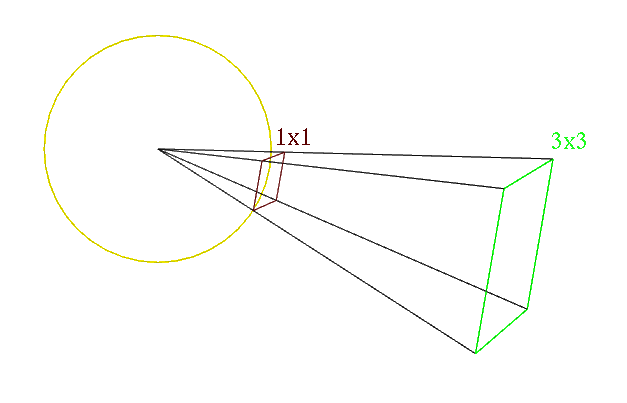
\includegraphics[width=0.5\textwidth]{expansion.png}
\EC

The larger green square is located three times further from the center than the smaller red one (which lies on the surface of the Sun). Since it is three times further away, it is also
three times taller and three times wider, as shown in the picture.

{\bf Question 2a:} How many times larger is the {\bf area} of the larger square than the smaller one?

\vspace*{2cm}

\hrulefill
\newpage
Now, imagine that the small square is on the surface of the Sun. The sunlight leaving the Sun, passing through the smaller, red square, 
will spread out until it reaches a distance three times 
the radius of the Sun (at the larger, green square.) If the intensity of the sunlight leaving the Sun is $I_1$, what do you expect the intensity of the sunlight to be once it reaches 
the outer square? (Hint: The sunlight is weaker because the same amount of light is spread over more area. How much more area?)

\vspace*{5cm}

\hrulefill

This last exercise involved looking at some example numbers; now, let's go back to our algebra. Here, instead of the ``large square'' (located at Earth) being three times further from the 
center than the ``small square'' (on the surface of the Sun), it is now $d/r$ times further away.


{\bf Question 2b:} In terms of $d$ and $r$, by what factor has the sunlight spread out by the time it reaches Earth?

\vspace*{5cm}

\hrulefill
\newpage
{\bf Question 2c:} In terms of $d$, $r$, and $I_1$ (the intensity of sunlight at the Sun's surface), write a formula for $I_2$ (the intensity of sunlight at Earth). 
Hint: Consider whether $d$ or $r$ is larger.
We expect $I_2$ to be much less than $I_1$; does your formula have this property? Call your TA over if you have questions; this is actually the trickiest part of this whole calculation.

\vspace*{5cm}

\hrulefill

When you are done with this section, ask your TA to check your results so far.

\subsection*{Method 2: More algebra, less reasoning}

We've talked so far about {\it intensity} -- the amount of power per unit area. If we multiply intensity by area, we can 
calculate the total power of the light passing through a certain area. In symbols, we know that $P=IA$.

Recall from your high school geometry class that the surface area of a sphere is $4\pi R^2$, where $R$ is the radius of 
the sphere.

Imagine two spheres. One lies just outside the surface of the Sun, and has radius $r$; the second lies
has its center is at the Sun and which is 1 AU in radius, so that the Earth (or other planet) 
is on its edge. (Its radius is $d$.) 

\begin{center}
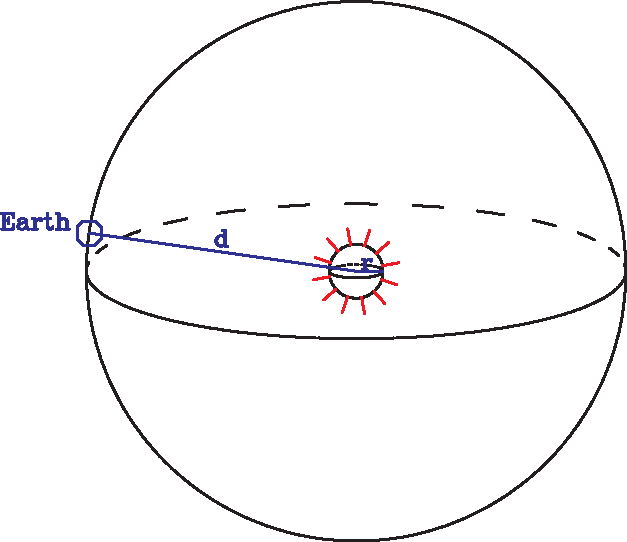
\includegraphics[width=3in]{expand-crop.pdf}
\end{center}

Call the surface area of the small sphere $A_1$ and the power of the sunlight passing through it $P_1$. Using the intensity/power 
relation above, this tells us that $P_1=I_1 A_1$. Likewise, call the surface area of the large sphere $A_2$, the power of the 
sunlight passing through it $P_2$, and the intensity of the light there $I_2$, and $P_2 = I_2 A_2$.

The key insight here is that the light from the Sun spreads out, but doesn't ``vanish'' as it travels through space. Thus,
the total power passing through both spheres is the same, and $I_1 A_1 = I_2 A_2$.

{\bf Question 3a:} Write expressions for $A_1$ and $A_2$ in terms of $r$ and $d$.

\vspace*{5cm}

\hrulefill


{\bf Question 3b:} Substitute the preceding expressions into $I_1 A_1 = I_2 A_2$ to arrive at an equation relating $d$, $r$,
$I_2$, and $I_1$.

\vspace*{5cm}

\hrulefill

{\bf Question 3c:} Solve the above for $I_2$ to get an expression for $I_2$, the intensity of sunlight at the Earth, in terms of
$d$, $r$, and $I_1$.
Hint: Consider whether $d$ or $r$ is larger.
We expect $I_2$ to be much less than $I_1$; does your formula have this property? Call your TA over if you have questions; this is actually the trickiest part of this whole calculation.
\vspace*{4cm}

\hrulefill




When you are done with this section, ask your TA to check your results so far.





\bigskip
\bigskip

{\bf Question 4:} Have you encountered anything else in this class that gets weaker proportional to the square of the distance from the Sun? Based on the geometry you did above, can you
think of why this might be the case?

\vspace*{4cm}

\hrulefill

{\bf Question 5:} One last thing: substitute the expression you found in Question 1 into the one you got for Question 2c or 3c. This should give you an expression for the intensity of
sunlight on the Earth, $I_2$, in terms of $d$, $r$, $k$, and $T_s$.

\vspace*{3cm}

\hrulefill


\section*{The thermal radiation of Earth}

{\bf Question 6:} If the Earth has a temperature $T_p$, what is the intensity of its outgoing thermal radiation $I_3$ in terms of $k$ and $T_p$? (This is again a straightforward application of the Stefan-Boltzmann law.)

\vspace*{3cm}

\hrulefill

\newpage
\section*{The temperature of Earth}

As discussed earlier, for Earth to be in balance, the same amount of light must flow in (from sunlight) and out (from Earth's thermal radiation). Na\"{i}vely, this would imply that
$I_2=I_3$. 

{\bf Question 7:} Equate the formulae you wrote for $I_2$ (in Question 5) and $I_3$ (in Question 6). Algebraically solve this equation for $T_p$, the temperature of the Earth. Ask your 
TA to check your result once you get it.

\vspace*{5cm}

\hrulefill

Now, finally, it's time to plug in numbers. Use the following:

\BI
\item $T_s$: 5700 K
\item $r$: 0.0046 AU
\item $d$: 1 AU
\EI


{\bf Question 8:} What estimate of the temperature of the Earth does this give you? (You will, as you might expect, need a calculator.)

\vspace*{2cm}

\hrulefill

{\bf Question 9:} Convert this value to Celsius or Fahrenheit. Is this a reasonably accurate value of the temperature of the Earth? Show your work to your TA.

\vspace*{4cm}

\hrulefill
\newpage

What has gone wrong here? We made an assumption that $I_3=I_2$ -- that is, that the {\it intensity of Earth's thermal radiation} must equal the {\it intensity of sunlight at Earth.}
This was a good first guess, and -- in a universe where things range from 3 Kelvin to millions of Kelvin -- it's not too bad. But we can do better!

The issue is that, really, we shouldn't be equating {\it intensities}; we should be thinking about the total {\it amount} of radiation. There are two ways we can improve our calculation:

\BI
\item Not all of the Earth is facing the Sun! The night half of Earth is still giving off thermal light; this implies that $I_3$ needs to be only half as big, since only half of 
Earth receives sunlight, but the entire Earth emits thermal radiation.
\item Remember how sunlight striking Earth at an angle doesn't heat it up as much, partially causing winter? This also reduces the amount of sunlight striking Earth's surface -- by
another factor of two. (The proof of this requires calculus.)
\EI

So, instead of writing $I_3 = I_2$, we can do better by writing $I_3 = \frac{1}{4} I_2$, since the Earth's shape means that the ``area that absorbs sunlight'' is only one-quarter
the area that emits thermal radiation. 

{\bf Question 10:} Set $I_3 = \frac{1}{4}I_2$ and solve this new equation for $T_p$. You should get an expression very similar to the one you got for Question 7.

\vspace*{4cm}

\hrulefill

{\bf Question 11:} Repeat your calculation for Earth's temperature with this new expression. Is your answer closer to the Earth's average surface temperature now? Is it too high, or 
too low?

\vspace*{4cm}

\hrulefill
\newpage


\section*{The temperatures of other planets}

Now, each of you in your lab group will individually repeat this calculation for a different planet. Use the following (minor) planets:

\BI
\item Venus, d=0.723 AU
\item Pluto, d=39.4 AU 
\item Mars, d=1.524 AU (groups of 3)
\EI

This should only require you to plug different values into the expression you got for Question 10. Each of you should do one planet, and share answers. 

\begin{enumerate}

\item Temperature of Venus:
\bigskip
\item Temperature of Pluto:
\bigskip
\item Temperature of Mars:
\bigskip

\end{enumerate}

Compare these results to the actual
temperatures of these planets' surfaces:

\BI
\item Earth: 288K / 59F
\item Mars: 218K / -67F 
\item Pluto: 44K / -380F
\item Venus: 735K / 864F
\EI

{\bf Question 12:} 
Venus is hotter than Earth; is this explained by the fact that it is closer to the Sun? Likewise, does the greater distance from the Sun explain the cooler temperatures on Mars?


\newpage

\section*{Wrapping a planet in glass}

As you saw in the demonstration with the infrared camera in class, glass (as in a student's eyeglasses) {\bf reflects infrared light}, but {\bf allows visible light} to pass.
Given that the Sun emits visible light but planets, with their lower temperatures, emit infrared light, what do you expect to happen to a planet's temperature if you were to
enclose it in a glass bubble? 

\bigskip
\bigskip
\bigskip
\bigskip
\bigskip

Other chemicals besides glass have this property as well -- some of them found in the atmospheres of planets. Earth has a moderately thick atmosphere, and Venus has a tremendously thick
atmosphere. Mars has almost no atmosphere at all. Note that your calculations on the previous page were off by 15 K for Earth, 3 K for Mars, and 400 K for Venus. 
What is going on here? 

\newpage
\section*{Other stars, other planets, and exterrestrial life}

One hopeful sign that there might be life on another planet would be for that planet to have a similar temperature to Earth. The star Sirius, the brightest in the night sky, 
has the following properties:

\BI
\item Radius: 0.008 AU (somewhat bigger than the Sun)
\item Surface temperature: 10,000 K
\EI

{\bf Question 12:} Take the formula you got in Question 10 and solve it instead for $d$. If a planet orbiting Sirius were to have the same temperature as Earth (about 288 K), 
how far from Sirius would its orbit be?

\end{document}
